%%%%%%%%%%%%%%%%%%%%%%%%
%
% $Author: Sadegh Naderi $
% $Datum: 2024-01-26  $
% $Pfad: ML23-01-Keyword-Spotting-with-an-Arduino-Nano-33-BLE-Sense\report\Contents\en\Data.tex $
% $Version: 3.0 $
% $Reviewed by: Sadegh Naderi $
% $Review Date: 2024-02-09 $
%
%%%%%%%%%%%%%%%%%%%%%%%%


\chapter{Data Description}
\label{chapter:DataDescription}

\section{Introduction}

The Speech Commands dataset aims to establish a standardized training and assessment dataset designed for straightforward speech recognition tasks. Its principal objective is to facilitate the development and testing of compact models capable of identifying instances when a specific word is uttered from a predefined set of ten words or fewer. The goal is to minimize false positives originating from background noise or irrelevant speech, a common challenge referred to as keyword spotting \cite{Warden:2018}.


\section{License}

In order to broaden its accessibility among researchers and developers, this dataset has been made available under the Creative Commons BY 4.0 license[5]. This allows for seamless integration into tutorials and scripts, enabling users to download and utilize it without the need for any user intervention, such as website registration or obtaining permission from an administrator via email. Additionally, the familiarity of this license in commercial contexts often expedites the approval process by legal teams when necessary \cite{Warden:2018}.

\section{Related Wok}

\href{https://commonvoice.mozilla.org/en}{Mozilla's Common Voice dataset} boasts over 500 hours of recordings from 20,000 diverse contributors and is released under the Creative Commons Zero license, akin to the public domain. This licensing structure facilitates easy integration and expansion. The dataset is sentence-aligned and was generated through volunteers reading requested phrases via a web application \cite{Warden:2018}.

LibriSpeech \cite{Panayotov:2015} comprises 1,000 hours of English speech, made available under the Creative Commons BY 4.0 license, and utilizes the widely supported open-source FLAC encoder for storage. Though labeled at the sentence level only, it lacks word-level alignment, making it more suitable for full automatic speech recognition rather than keyword spotting \cite{Warden:2018}.

\href{https://catalog.ldc.upenn.edu/docs/LDC93S10/tidigits.readme.html}{TIDIGITS} encompasses 25,000 digit sequences spoken by 300 contributors in a quiet environment. This dataset is exclusively accessible under a commercial license from the Language Data Consortium and is stored in the NIST SPHERE file format, posing challenges in decoding with modern software. Initial experiments on keyword spotting were conducted using this dataset \cite{Warden:2018}.


\section{Dataset Characteristics, Collection and Origin}

The distinctions between on-device keyword spotting and general speech recognition models lead to significant differences in their training and evaluation processes. While datasets like Mozilla's Common Voice show promise for general speech tasks, their adaptability to keyword spotting is challenging \cite{Warden:2018}. Some characteristics of the data are:

\begin{itemize}
	\item Realistic Audio Capture
	
	\begin{itemize}
		\item Avoiding the use of studio-captured samples. Reasons:
		\begin{itemize}
			\item Absence of background noise in the audio
			\item Recorded with high-quality microphones
		\end{itemize}
	\end{itemize}
	
	\item Recorded using phone or laptop microphones
	\item Language focus: English
	\item Audio format: WAV
	\item Various accents in addition to American English
	\item Several individuals are recorded (to ensure speaker independence)
	\item One second single words
	\item Sample rate (frequency) set to 16 KHz
	\item Download size: 2.37 GB
	\item Dataset size: 8.17 GB
	\item Subset of the dataset used: 415 MB
	\item Open-source
	\item Anonymous
	\begin{itemize}
		\item Recording personally identifiable information was avoided
	\end{itemize}
\end{itemize}

Using studio-captured samples appeared impractical due to the absence of background noise, high-quality microphones, and a formal setting. Successful models needed to handle noisy environments, low-quality recording equipment, and natural, casual conversation. To address this, all utterances were recorded using phone or laptop microphones in various user locations. The only exception was when users were requested to be alone in a closed room to avoid background conversations for privacy reasons \cite{Warden:2018}.

Aiming to counter the common bias towards American English prevalent in many voice interfaces, a wide variety of accents was sought to be gathered \cite{Warden:2018}.

Another objective was to have as many different people recorded as possible. Speaker independence significantly enhances the utility of keyword-spotting models \cite{Warden:2018}.

The avoidance of recording any personally identifiable information from contributors was also desired, given that extreme care is required for handling such data due to privacy reasons. This involved refraining from requesting attributes like gender or ethnicity, not mandating a sign-in through a user ID that could link to personal data, and necessitating users to agree to a data-usage agreement before contributing \cite{Warden:2018}.

To streamline the training and evaluation process, the decision was made to confine all utterances to a standardized duration of one second. This involves excluding longer words, but given that the typical targets for keyword recognition are short, this restriction did not appear excessively limiting. Furthermore, it was determined to exclusively capture single words spoken in isolation, as opposed to within sentences. This choice closely aligns with the targeted trigger word task and simplifies the labeling process, as alignment becomes less crucial \cite{Warden:2018}.

To download the dataset: \texttt{\url{https://storage.googleapis.com/download.tensorflow.org/data/speech\_commands\_v0.02.tar.gz}}

\section{Selection of Words}

Decision was made to maintain a limited vocabulary for the purpose of ensuring a lightweight capture process, while still incorporating sufficient variety for potential usefulness in certain applications by models trained on the data. This led to the selection of twenty common words as the core vocabulary, encompassing digits zero to nine and ten additional words suitable for IoT or robotics commands: "Yes," "No," "Up," "Down," "Left," "Right," "On," "Off," "Stop," "Go," "Backward," "Forward," "Follow," and "Learn." Addressing a key challenge in keyword recognition, a set of words was needed to act as tests for the ability to ignore speech lacking triggers. Some, like "Tree," were chosen for their phonetic similarity to target words, serving as tests for a model's discernment, while others were arbitrarily selected as short words covering various phonemes, resulting in the final list: "Bed," "Bird," "Cat," "Dog," "Happy," "House," "Marvin," "Sheila," "Tree," and "Wow." The final list of all the utterances is shown in Table \ref{tab:utterances}.

\begin{table}[ht]
	\centering
	\caption{Number of Utterances for Each Word \cite{Warden:2018}}
	\label{tab:utterances}
	\begin{tabular}{clc}
		\textbf{Index} & \textbf{Word} & \textbf{Number of Utterances} \\
		\hline
		1 & Backward & 1,664 \\
		2 & Bed & 2,014 \\
		3 & Bird & 2,064 \\
		4 & Cat & 2,031 \\
		5 & Dog & 2,128 \\
		6 & Down & 3,917 \\
		7 & Eight & 3,787 \\
		8 & Five & 4,052 \\
		9 & Follow & 1,579 \\
		10 & Forward & 1,557 \\
		11 & Four & 3,728 \\
		12 & Go & 3,880 \\
		13 & Happy & 2,054 \\
		14 & House & 2,113 \\
		15 & Learn & 1,575 \\
		16 & Left & 3,801 \\
		17 & Marvin & 2,100 \\
		18 & Nine & 3,934 \\
		19 & No & 3,941 \\
		20 & Off & 3,745 \\
		21 & On & 3,845 \\
		22 & One & 3,890 \\
		23 & Right & 3,778 \\
		24 & Seven & 3,998 \\
		25 & Sheila & 2,022 \\
		26 & Six & 3,860 \\
		27 & Stop & 3,872 \\
		28 & Three & 3,727 \\
		29 & Tree & 1,759 \\
		30 & Two & 3,880 \\
		31 & Up & 3,723 \\
		32 & Visual & 1,592 \\
		33 & Wow & 2,123 \\
		34 & Yes & 4,044 \\
		35 & Zero & 4,052 \\
		\hline
	\end{tabular}
\end{table}


\section{Quality Control}
\label{section:QC}

Criteria were needed to accept or reject submissions due to the variable quality of the gathered audio utterances. An informal guideline was applied, where clips that were indiscernible to a human listener or sounded like incorrect words were slated for \cite{Warden:2018}.

To eliminate extremely short or quiet clips, the nature of the OGG compression format was leveraged. Clips with minimal audio content had significantly smaller file sizes, and a heuristic was established to reject files smaller than 5 KB \cite{Warden:2018}.

Subsequently, the OGG files were transformed into uncompressed WAV files containing PCM sample data at 16KHz, as this format facilitates further processing \cite{Warden:2018}.

Samples from other sources, which arrived as WAV files with varying sample rates, were also resampled to 16 KHz WAV files \cite{Warden:2018}.


\section{Capture the Loudest Segment}
\label{section:CaptureLoudest}

The existence of a considerable number of utterances that were too quiet or entirely silent was noted during manual inspection of the samples gathered. The alignment of spoken words within the 1.5-second file was found to be arbitrary, depending on the user's response speed to the displayed word. To address both issues, a simple audio processing tool was created to assess the overall volume of the clips \cite{Warden:2018}.

In the initial stage, the absolute differences of all the samples from zero were summed, using a scale where -32768 in the 16-bit sample data represented -1.0 as a floating-point number, and +32767 was 1.0. The mean average of this value was examined to estimate the overall volume of the utterance. Through experimentation, it was determined that anything below 0.004 on this metric was likely too quiet to be intelligible, leading to the removal of such clips \cite{Warden:2018}.

To approximate the correct alignment, the tool then extracted the one-second clip containing the highest overall volume. This approach tended to center the spoken word in the middle of the trimmed clip, assuming that the utterance was the loudest part of the recording \cite{Warden:2018}.

\section{Release Procedure}

The recorded utterances were organized into individual folders, each corresponding to a specific word. The original 16-digit hexadecimal speaker ID numbers present in the web application's file names were hashed into 8-digit hexadecimal IDs. Speaker IDs from other sources, such as paid crowdsourcing sites, were similarly hashed into the same format. This was done to eliminate any link to worker IDs or other personally identifiable information. While the hash function used is stable, ensuring consistency, the IDs for existing files should remain unchanged in future releases even with the addition of more speakers \cite{Warden:2018}.

\section{Background Noise}

A crucial requirement for keyword spotting in real products is the ability to differentiate between audio containing speech and clips devoid of speech. To aid in training and testing this capability, several minute-long 16 KHz WAV files of various types of background noise were incorporated. Some of these were directly recorded from noisy environments, such as those near running water or machinery, while others were mathematically generated using Python. In order to differentiate these files from word utterances, they were placed within a designated \texttt{"\_background\_noise\_"} folder located at the root of the archive \cite{Warden:2018}.

\section{Potential Anomalies in the Dataset}

In the preceding sections, we discussed the handling of anomalies. This section provides a summary of potential anomalies that could be introduced in such datasets. Some common anomalies or challenges might include:

\subsubsection{Background Noise Variability}

\begin{itemize}
	\item \textbf{Anomaly:} Inconsistencies in background noise levels or types across different recordings.
	\item \textbf{Challenge:} Ensuring the model can effectively distinguish between target keywords and various background noises.
\end{itemize}

\subsubsection{Accents and Pronunciation}

\begin{itemize}
	\item \textbf{Anomaly:} Presence of diverse accents or variations in pronunciation.
	\item \textbf{Challenge:} Ensuring the model's robustness to different accents and pronunciations, preventing bias towards specific linguistic patterns.
\end{itemize}

\subsubsection{Recording Quality}

\begin{itemize}
	\item \textbf{Anomaly:} Variability in recording quality, including low-quality or noisy recordings.
	\item \textbf{Challenge:} Developing a model that performs well on recordings from different devices and environments.
\end{itemize}

\subsubsection{Speaker Characteristics}

\begin{itemize}
	\item \textbf{Anomaly:} Differences in speaker characteristics such as pitch, speed, or age.
	\item \textbf{Challenge:} Designing a model that generalizes well across various speaker attributes.
\end{itemize}

\subsubsection{Imbalanced Dataset}

\begin{itemize}
	\item \textbf{Anomaly:} Significant variations in the number of instances for different keywords.
	\item \textbf{Challenge:} Ensuring a balanced dataset to prevent the model from being biased toward more frequently occurring keywords.
\end{itemize}

\subsubsection{Unintended Triggers}

\begin{itemize}
	\item \textbf{Anomaly:} Instances where unintended words or sounds trigger the keyword spotting.
	\item \textbf{Challenge:} Implementing measures to minimize false positives caused by words with phonetic similarities or ambiguous sounds.
\end{itemize}

\subsubsection{Inconsistent Recording Conditions}

\begin{itemize}
	\item \textbf{Anomaly:} Changes in recording conditions, such as recording in a noisy environment for some words and a quiet room for others.
	\item \textbf{Challenge:} Ensuring the model's ability to handle diverse recording conditions.
\end{itemize}

\subsubsection{Data Privacy Concerns}

\begin{itemize}
	\item \textbf{Anomaly:} Accidental inclusion of personally identifiable information in recordings.
	\item \textbf{Challenge:} Implementing strict protocols to ensure privacy and anonymizing data appropriately.
\end{itemize}

\subsubsection{Unexpected Word Variations}

\begin{itemize}
	\item \textbf{Anomaly:} Variability in word variations (e.g., different verb tenses, plural forms).
	\item \textbf{Challenge:} Creating a model that recognizes variations of target words.
\end{itemize}

\subsubsection{Mislabeling or Incorrect Annotations}

\begin{itemize}
	\item \textbf{Anomaly:} Instances where labels or annotations do not accurately represent the content.
	\item \textbf{Challenge:} Implementing rigorous quality control to identify and rectify mislabeled instances.
\end{itemize}


\section{How to Record your Own voice}

\begin{figure}[h!]
	\centering
	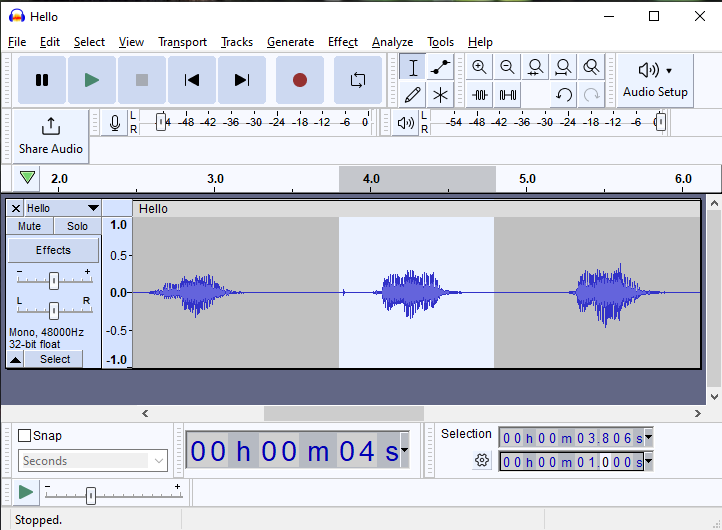
\includegraphics[width=0.8\textwidth]{Images/Data/EditRecordedinAudacity}
	\caption{Audacity user interface} \label{fig:Audacity}
\end{figure}

\begin{enumerate}
	\item Record your voice using a recording device.
	\item Change the format to WAV.
	\item Use Audacity for editing.
	\item Set the project rate to 16kHz.
	\item Resample the entire recording to match the 16kHz sample rate.
	\item Select one second of audio.
	\item Export each second of audio as a WAV file. Use 32-bit float as the encoding, matching the bit depth of other samples.
	\item The file name can be chosen according to one's own preferences.
	\item Create a new folder and name it after your keyword (e.g., "Hello").
	\item Move all the samples to this folder.
	\item Place the folder alongside other sample keyword folders.
	\begin{itemize}
		\item prevent bias
	\end{itemize}
\end{enumerate}

\subsubsection{Aim for a Balanced Dataset to Avoid Bias}

Note that the aim should be set for a balanced dataset. For example a dataset where each class or category of interest has approximately the same number of instances. This is particularly important when training a model, as an imbalanced dataset may lead the model to be biased toward the majority class, potentially hindering its ability to generalize well to minority classes.

For example, if you're training a model to recognize different accents, having a balanced dataset would mean ensuring that you have a similar number of examples for each accent you want the model to identify. This helps prevent the model from becoming overly influenced by the accent with the most instances and allows it to learn patterns from all classes more effectively.


\subsection{How to Install Audacity}

\subsubsection{Windows:}

\begin{enumerate}
	\item Visit the official Audacity website: \texttt{https://www.audacityteam.org/}
	\item Navigate to the "Download" section.
	\item Click on the Windows logo to download the installer for Windows.
	\item Run the downloaded installer file.
	\item Follow the on-screen instructions to complete the installation.
\end{enumerate}

\subsubsection{macOS:}

\begin{enumerate}
	\item Visit the official Audacity website: \texttt{https://www.audacityteam.org/}
	\item Navigate to the "Download" section.
	\item Click on the Apple logo to download the installer for macOS.
	\item Open the downloaded DMG file.
	\item Drag the Audacity application to your Applications folder.
\end{enumerate}

After installation, you can launch Audacity and start using it for audio editing.

\subsection{License of Audacity Software Product}

Audacity is released under the GNU General Public License (GPL). Specifically, Audacity is licensed under the GNU GPL version 2 or later. The GPL is a free software license that allows users to run, study, modify, and distribute the software and its source code.


\section{How to Train a more Robust Model}

\begin{itemize}
	\item Add more background noise situations
	\item More different accents
	\item More different vocal ranges
	\item More different timbres (tones)
	\begin{itemize}
		\item Keep in mind that air acts as a dispersive medium, introducing variations in the timbre (tone) of sounds produced by individuals singing at the same frequency (pitch). For instance, a note played on a piano exhibits a distinct timbre compared to the same note played on a guitar.
	\end{itemize}
	\item Different recording devices
	\item Variable speed
	\item Data augmentation techniques
	\begin{itemize}
		\item e.g., Pitch shifting
		\item e.g., Time stretching
	\end{itemize}
	\item  Different ages
	\begin{itemize}
		\item For instance, the voices of elderly individuals often exhibit tremors.
	\end{itemize}
\end{itemize}

